%%%%%%%%%%%%%%%%%%%%%%%%%%%%%%%%%%%%%%%%%
% Adapted from: Beamer Presentation, LaTeX Template, Version 1.0 (10/11/12), http://www.LaTeXTemplates.com
%%%%%%%%%%%%%%%%%%%%%%%%%%%%%%%%%%%%%%%%%
% DATE: 2019-08-12
% AUTHORS:
% Sebastian Steffen
%%%%%%%%%%%%%%%%%%%%%%%%%%%%%%%%%%%%%%%%%
% TODO:
%%%%%%%%%%%%%%%%%%%%%%%%%%%%%%%%%%%%%%%%%

%----------------------------------------------------------------------------------------
%	PACKAGES AND THEMES
%----------------------------------------------------------------------------------------

\documentclass[12pt,aspectratio=169]{beamer}

\mode<presentation> {
\usetheme{Boadilla}
%\setbeamertemplate{footline} % To remove the footer line in all slides uncomment this line
%\setbeamertemplate{footline}[page number] % To replace the footer line in all slides with a simple slide count uncomment this line

%\setbeamertemplate{navigation symbols}{} % To remove the navigation symbols from the bottom of all slides uncomment this line
}

\usepackage{graphicx} % Allows including images
\usepackage{booktabs} % Allows the use of \toprule, \midrule and \bottomrule in tables
\usepackage{hyperref} % Make Urls Blue
\usepackage[savemem]{listings} % For code blocks
\usepackage{comment}
\usepackage{xcolor} % for colors
\hypersetup{
urlcolor=cyan, 
colorlinks=true, 
citecolor=green, 
linkcolor=red,
filecolor=magenta     
}
\urlstyle{same}

%\usepackage{pgfpages} % To render notes side by side with slides.

\newenvironment{wideitemize}{\itemize\addtolength{\itemsep}{10pt}}{\enditemize}

%\setbeameroption{show notes on second screen}
%\setbeameroption{show only notes} % Use this to only show notes for easy printing of the notes.
\setbeameroption{hide notes} % This is the default for easy printing of the slides.

%----------------------------------------------------------------------------------------
%	TITLE PAGE
%----------------------------------------------------------------------------------------
\title[A-Lab]{A-Lab Tutorial \\ Data Wrangling and Visualization in R} % The short title (first) appears at the bottom of every slide, the full title (second) is only on the title page

\author{} % Your name
\institute[] % Your institution as it will appear on the bottom of every slide, may be shorthand to save space
{
Sebastian Steffen \\ % Your institution for the title page
\medskip
\textit{ssteffen@mit.edu} % Your email address
}
\date{\today} % Date, can be changed to a custom date

\begin{document}

\begin{frame}
\titlepage % Print the title page as the first slide
\end{frame}

\begin{frame}
\frametitle{Overview} % Table of contents slide, comment this block out to remove it
\tableofcontents % Throughout your presentation, if you choose to use \section{} and \subsection{} commands, these will automatically be printed on this slide as an overview of your presentation
\end{frame}

\AtBeginSection[]
{
\begin{frame}<beamer>
\frametitle{Workshop Outline}
\tableofcontents[currentsection]
\end{frame}
}

%----------------------------------------------------------------------------------------
%	PRESENTATION SLIDES
%----------------------------------------------------------------------------------------

\section{Teaching Learning Objectives (TLOs)}
\begin{frame}{Teaching Learning Objectives (TLOs)}
\begin{itemize}
    \item<1-> Install and Set Up R and tidyverse.
    \item<2-> Understand key data concepts. 
    \item<3-> Know vocabulary and libraries for better search queries.
    \item<4-> Overview of the basics.
    \item<5->[]
    \item<5-> Ultimate Goal is to help you help yourself.
    \item<6-> Q\&A.
\end{itemize}
\end{frame}

\begin{frame}{Before We Begin..}
 Please take a few minutes to think about the data for your own project (alternatively, do this once you have access to it):
\begin{itemize}
    \item<1-> Which questions do you have to answer? Which can you answer? Which do you want to answer? Why are they important? List a few.
    \item<2-> What would the ideal data look like? What variables would you need? What format does the data need to be in (i.e. what should each row look like)?
    \item<3-> What are your hypotheses?
    \item<4-> What method do you need to apply?
    \item<5-> Is there prior work (i.e. literature, news, \dots) that attempts to answer it that you can leverage?
\end{itemize}
\end{frame}

\begin{frame}{Example}
Want to understand the value of different skills.
Long history in Economics on estimating the 'Returns to "Skill"'.
    \begin{itemize}
        \item How valuable is learning to code? What's the \$-value associated with R?
        \item My Research: What skills do employers demand and how much are they willing to pay.
        \item Ideal data: Panel data of job postings annotated with skills demanded and employer. Each row is a bundle of skills and a \$-value (wage).
        \item Hypothesis: Value of coding is high and has increased over time.
        \item Method: OLS Regression (for interpretability) with employer fixed effects
        \item[]
        \item Conversely, if I wanted to predict the future value of R, I'd instead need a time series of \$-values for R and might use ARIMA.
    \end{itemize}
\end{frame}

\begin{frame}{Data Wrangling}
\begin{block}{\textbf{Data Wrangling}}
Methods to transform raw data into usable a format to answer a specific research question.
\end{block}
\begin{itemize}
    \item Different research questions require different data formats.
\end{itemize}
\end{frame}



\section{Boring Stuff}
\begin{frame}{Installation of R}
\begin{itemize}
    \item R: \url{https://cloud.r-project.org/}
    \item RStudio Desktop IDE: \url{https://www.rstudio.com/products/rstudio/download/}
    \item Install packages via 'Tools' or via \texttt{install.packages(<package\_name>)}:
    \begin{itemize}
    \item tidyverse
    \begin{itemize}
        \item includes several extremely useful packages: tidyr, dplyr, purrr, stringr, forcats, lubridate, ggplot2
    \end{itemize}
    \item  \dots
    \item mice, tidytext, philentropy, lfe, rpart, causaltree, glmnet, fuzzywuzzy, shinyr, nnet, neuralnet, tensorflow, sf, \dots
    \end{itemize}
\end{itemize}
\begin{figure}
\centering
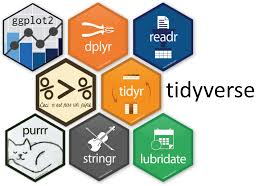
\includegraphics[width=1.0\linewidth,height=0.3\textheight,keepaspectratio]{resources/tidyverse-2.jpeg}
\end{figure}
\end{frame}

\begin{frame}{Project Environment Tips}
\begin{wideitemize}
\item<1-> Keep project folder organized (i.e. via \href{https://web.stanford.edu/~gentzkow/research/CodeAndData.pdf}{Gentzkow, Shapiro (2014)}).
\item<2-> Never change the raw data - always work on a copy!
\item<3-> Try to use functional programming for any task you do more than twice. (a bit of a learning curve with dplyr $\rightarrow$href{https://dplyr.tidyverse.org/articles/programming.html}{quosures})
\item<4-> Use (Jupyter) Notebooks to explore data. Later, move to automating stuff via command line and \texttt{screen} (or batch files, i.e. on Sloan's Engaging Server).
\end{wideitemize}
\end{frame}

\section{Concepts}
\begin{frame}{Tidy Data}
\begin{itemize}
    \item<1-> \textbf{Every column is a variable.}
    \item<2-> \textbf{Every row is an observation.}
    \item<3-> \textbf{Every cell is a single value.}
\end{itemize}
\only<1>
{
NOT
\begin{table}[]
\begin{tabular}{lll}
brand\_model & year & mileage \\
\hline
Audi\_A4 & 1999 & 18      \\
Audi\_A4 & 2008 & 20      \\
VW\_GTI  & 1999 & 19      \\
VW\_GTI  & 2008 & 22      \\
...     & ...  & ...    
\end{tabular}
\end{table}
\begin{itemize}
    \item Can be fixed with \texttt{separate()}.
\end{itemize}
}
\only<2>
{
NOT
\begin{table}[]
\begin{tabular}{llll}
brand & model & mileage\_1999 & mileage\_2008 \\
\hline
Audi    & A4    & 18 & 20      \\
VW      & GTI   & 19 & 22      \\
...   & ...  & ...    
\end{tabular}
\end{table}
\begin{itemize}
    \item Can be fixed with \texttt{pivot\_longer()}, \texttt{pivot\_wider()} (formerly \texttt{gather()}, \texttt{spread()}).
\end{itemize}
}
\only<3>
{
\begin{table}[]
\begin{tabular}{lll}
brand & model & mileages\_1999\_2008 \\
\hline
Audi  & A4    & (18, 20)      \\
VW    & GTI   & (19 , 22)    \\
...   & ...   & ...  
\end{tabular}
\end{table}
\begin{itemize}
    \item Can be fixed with \texttt{separate()} and \texttt{pivot\_longer()}. 
\end{itemize}
}
\only<4>
{
\begin{table}[]
\begin{tabular}{lll|ll}
\textbf{brand} & \textbf{model} & \textbf{year} & mileage & \dots \\
\hline
Audi  & A4    & 1999 & 18 & \dots     \\
Audi  & A4    & 2008 & 20 & \dots     \\
VW    & GTI   & 1999 & 19 & \dots     \\
VW    & GTI   & 2008 & 22 & \dots     \\
VW    & GTI   & 2012 & 24 & \dots     \\
Mazda & CX-5  & 2017 & 23 & \dots     \\
...   & ...   & ...  & ...& \dots  
\end{tabular}
\end{table}
\begin{itemize}
    \item Tidy data: Each row has a \textbf{unique key (or index)} and \textbf{values}.
    \item Here, the key/index is \textbf{brand x model x year}, values are mileage.
\end{itemize}
}
\end{frame}

\begin{frame}{Tidy Data - Easier Said than Done}
    \begin{itemize}
        \item<1-> Example I: Which car has the lowest fuel consumption?
        \item<2-> Example II: Which car brand is the most innovative (in terms of updated models)?
        \item<3-> Example III: Predict average fuel consumption in 2016.
        \item<4->[]
        \item<4-> Definition of clean data depends on the question(s). $\rightarrow$ Need to know how to transform one data format into another.
    \end{itemize}
\end{frame}

\section{R and Tidyverse Crashcourse}
\begin{frame}{Chaining with Pipes}
\begin{itemize}
    \item Pipes let you read code from left to right by chaining commands together. $\rightarrow$ More legible code. 
\end{itemize}

\begin{table}[]
    \centering
    \begin{tabular}{|c|c|}
    \hline
    Without Chaining & With Chaining \\
    \hline
    f(x)  &  x $\rightarrow$ f \\
    f(x, y) & x $\rightarrow$ f(y) \\
    f(g(x)) & x $\rightarrow$ f $\rightarrow$ g \\
    \hline
    \end{tabular}
\end{table}
\end{frame}

\begin{frame}{Basic Operations}
    \begin{itemize}
        \item \texttt{filter}: filter data based on logical condition.
        \item \texttt{mutate}: create new (and change old) variables.
        \item \texttt{group\_by, ungroup()}: define (temporary) keys.
        \item \texttt{summarize}: Used with \texttt{group\_by} to aggregate columns.
        \texttt{arrange}: reorder rows (i.e. sort).
        \texttt{select}: subset (and reorder) columns.
    \end{itemize}
\end{frame}

\begin{frame}{Quick Example}
Common Operations
    \begin{itemize}
        \item Log: $log(x+1)$
        \item \%-Change over time: $group\_by(Group) \%>\% arrange(-T) \%>\% mutate(Change = last(X)/first(X) - 1$
        \item 
    \end{itemize}
\end{frame}

\begin{frame}{More Advanced Words}
\begin{itemize}
    \item \texttt{\href{https://dplyr.tidyverse.org/reference/across.html}{across}} (supersedes \texttt{mutate\_at} and \texttt{mutate\_if}).
    \item \texttt{\href{https://tidyr.tidyverse.org/reference/pivot_longer.html}{pivot\_longer}, \href{https://tidyr.tidyverse.org/reference/pivot_wider.html}{pivot\_wider}}: Make dataset longer or wider (i.e. from time series to panel or vice versa).
\end{itemize}
\end{frame}

\begin{frame}{Types of Data}
   \begin{itemize}
   \item Cross-Sectional Data: Many subjects, one point in time.       
   \item Time Series: One subject, many points in time.
   \item Panel Data: Many subjects, many points in time. May be unbalanced, i.e. some (subject, time) combinations are missing.
   \item Multidimensional Panel Data: More than 2 dimensions, i.e. (subject, time, group)
   \end{itemize} 
\end{frame}

\begin{frame}{Long versus Wide Data}
    \begin{figure}
        \centering
        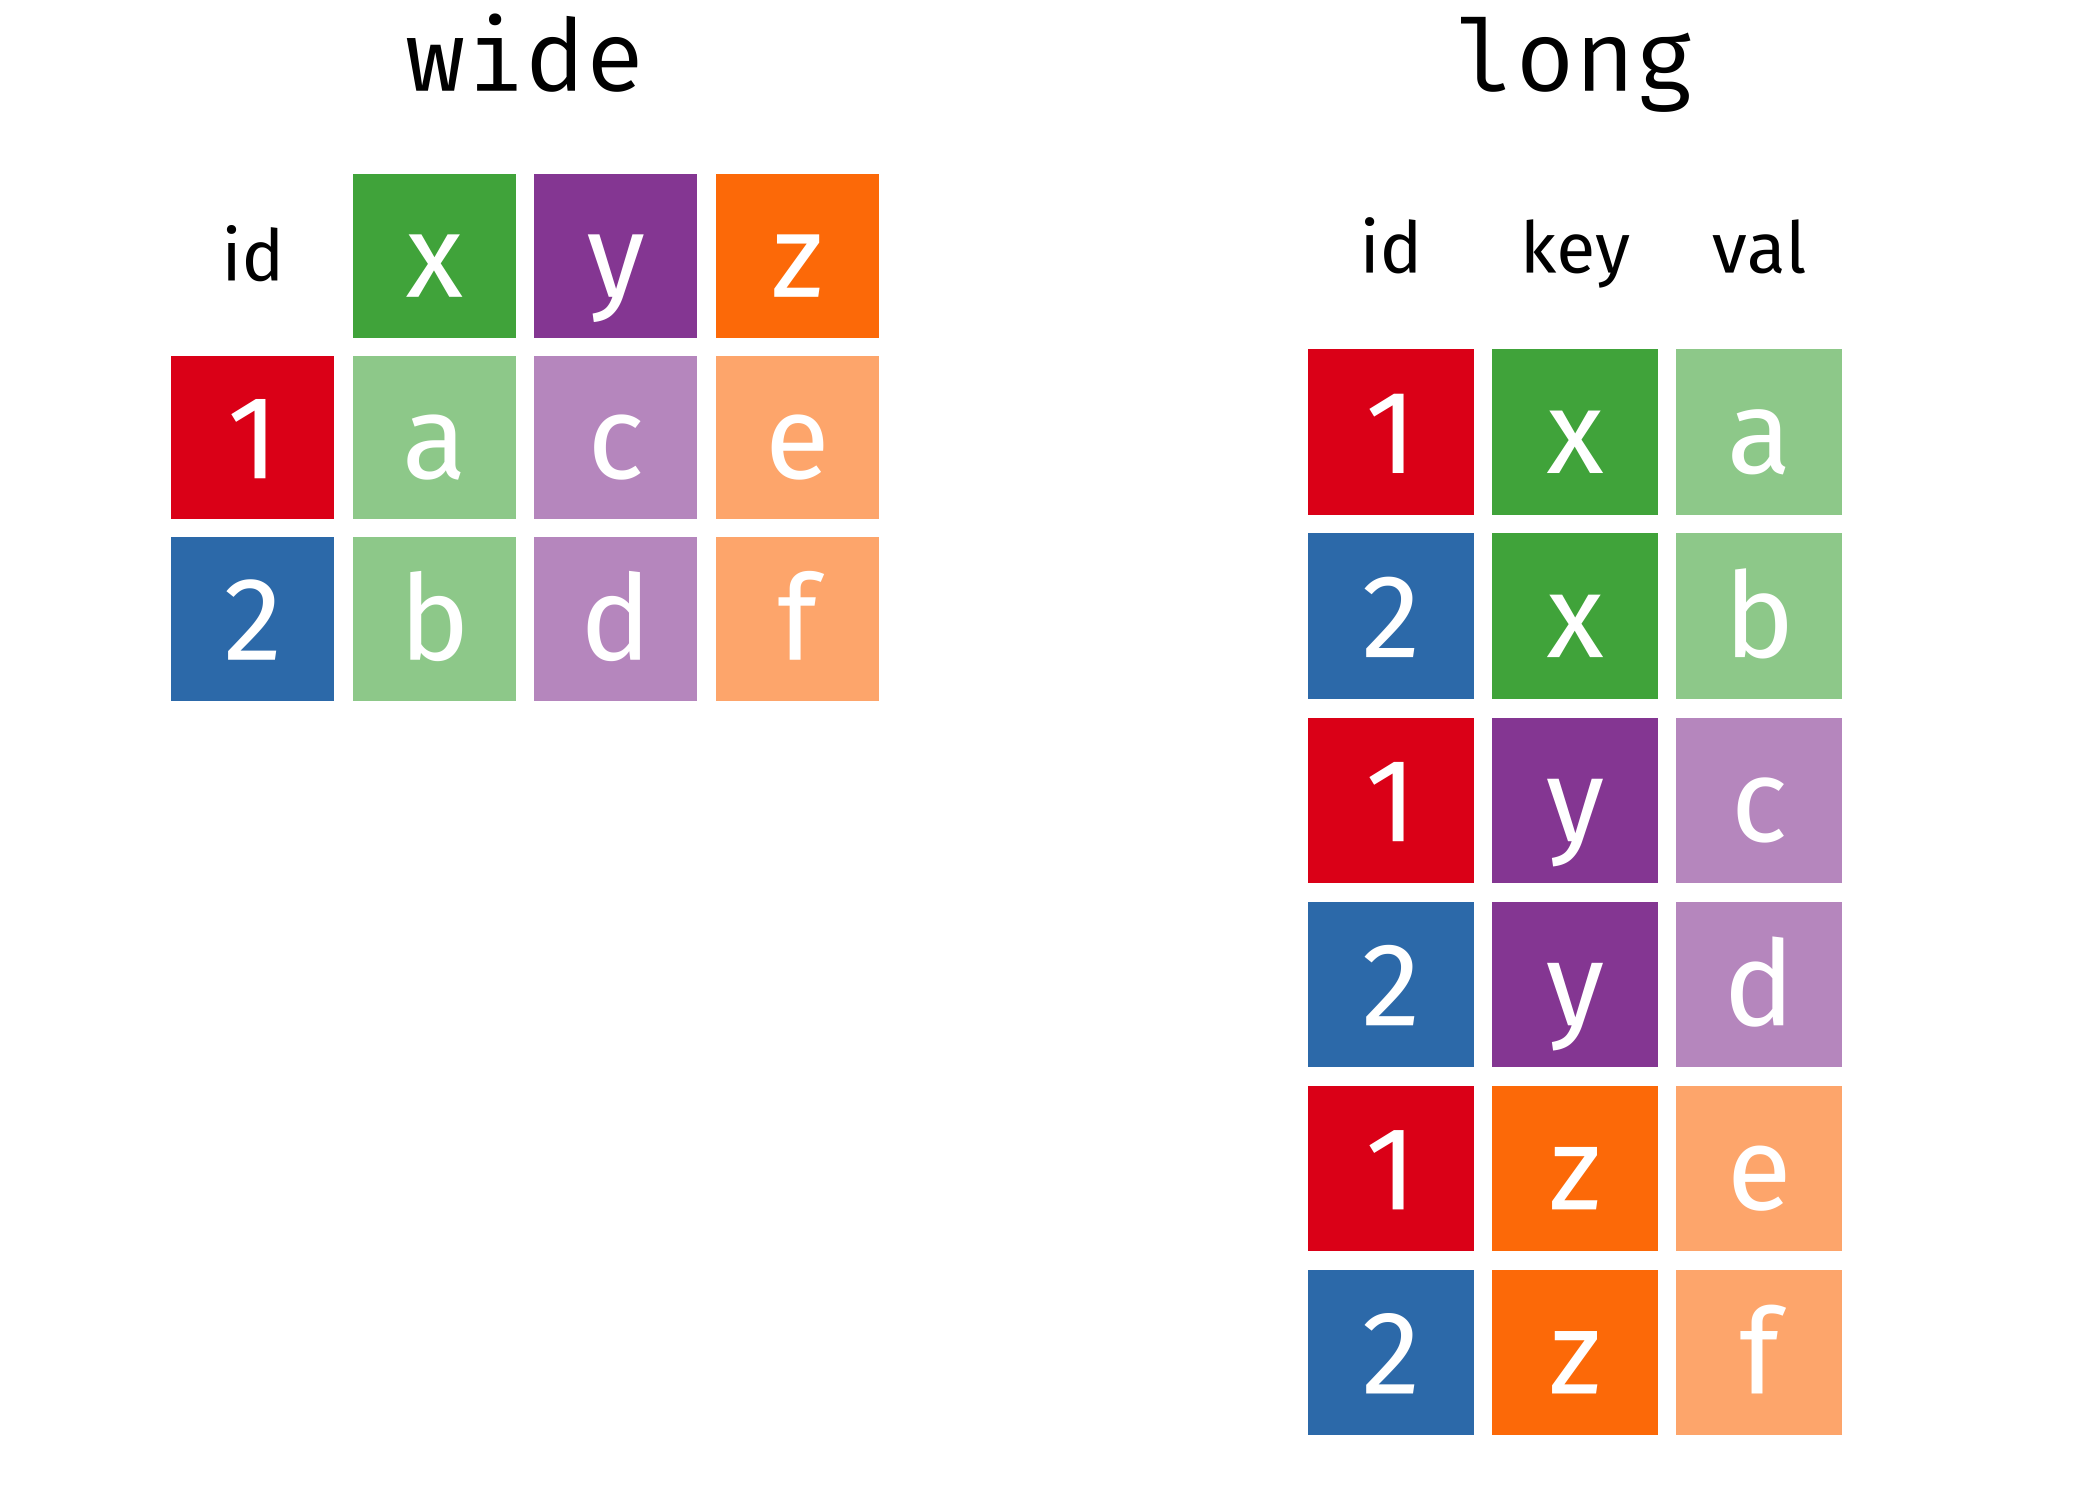
\includegraphics[width=0.8\textwidth,height=0.8\textheight,keepaspectratio]{resources/wide_long_data.png}
        \end{figure}
        \begin{itemize}
            \item The first allows analyses at the id (1, 2) level, the second at the id, key level.
        \end{itemize}
\end{frame}

\begin{frame}{Aggregation}
    \begin{wideitemize}
        \item Groups/Reduces multiple rows into one:
        \item \texttt{df <- cars \%$>$\% group\_by(brand, year) \%$>$\% summarize(num\_models = n(), mean\_mpg = mean(mpg, na.rm = TRUE)}
        \item Common Aggregation functions: \texttt{mean(), sd(), first(), last(), sum(), min(), max(), n()}
    \end{wideitemize}
\end{frame}

\begin{frame}{Joins/Merges and Appends}
  \begin{columns}[c]
        \column{.5\textwidth} % Left column and width
        \begin{itemize}
            \item Append: Requires same column names (\texttt{\href{https://dplyr.tidyverse.org/reference/bind.html}{bind\_rows()}, bind\_cols()}
            \item Join/Merge: Requires key to identify matching rows.
            \begin{itemize}
                \item Left Outer Join: Keep all (including unmatched) rows from left. (\texttt{left\_join}).
                \item Inner Join: Only keep matching rows (\texttt{inner\_join()}).
                \item Anti Join: Only keep unmatched rows from left (\texttt{anti\_join()}).
                \item Full Join: Keep all rows from both left and right (\texttt{full\_join()}).
            \end{itemize}
        \end{itemize}
        \column{.5\textwidth} % Right column and width
        \begin{figure}
        \centering
        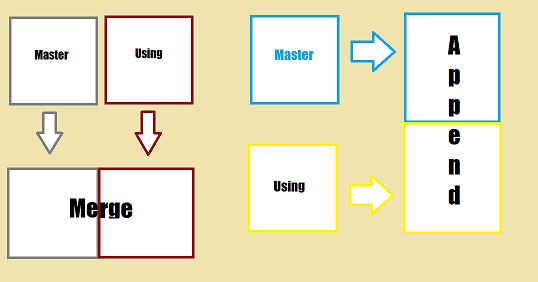
\includegraphics[width=1.0\linewidth,height=0.6\textheight,keepaspectratio]{resources/merge_append_data.png}
        \end{figure}
    \end{columns}
\end{frame}

\begin{frame}{Join Types Visualized}
    \begin{figure}
        \centering
        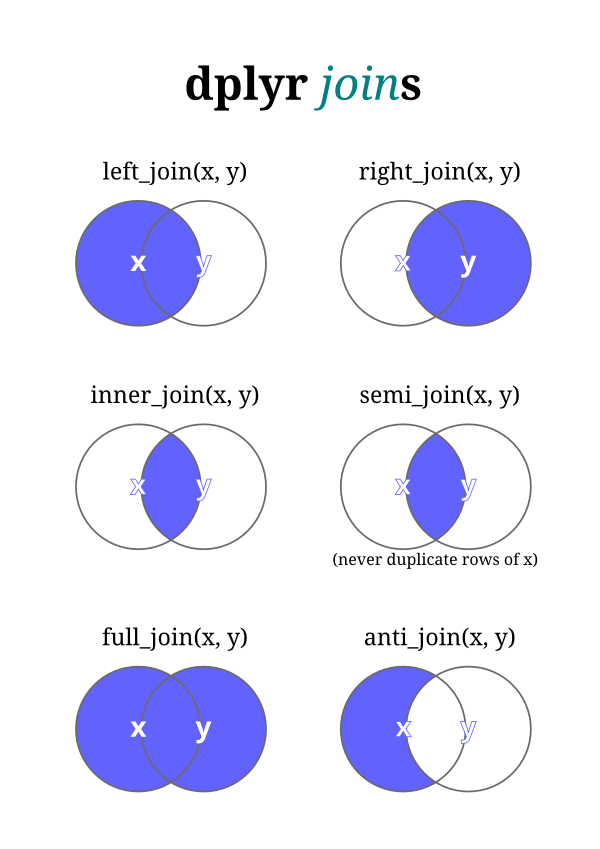
\includegraphics[width=0.8\linewidth, height=0.8\textheight, keepaspectratio]{resources/dplyr_joins.png}
    \end{figure}
\end{frame}

\begin{frame}{Package Overview}
\resizebox{\linewidth}{!}{
        \begin{tabular}{l|ll}
        Type & R & Python \\
        \hline \\
        Missing Values  & \texttt{mice}                     & \texttt{fancyimpute, statsmodels} \\
        Data Wrangling  & \texttt{dplyr}                    & \texttt{pandas} \\
        Strings         & \texttt{stringr}                  & built-in, \texttt{pandas} \\
        (Fuzzy) String Matching & \texttt{fuzzywuzzyR}      & \texttt{fuzzywuzzy} \\
        Dates           & \texttt{lubridate}                & built-in, \texttt{pandas} \\
        Geographical    & \texttt{ggmap, maps, maptools}    & \texttt{geopandas} \\
        Visualization   & \texttt{ggplot2, bokeh}           & \texttt{plotnine, bokeh, matplotlib} \\
        Regressions (with p-values)     & \texttt{lm, lfe}                  & \texttt{statsmodels} \\
        Machine Learning                & \texttt{caret, glmnet, rpart}     & \texttt{scikit-learn} \\
        Deep Learning   &  t\texttt{tensorflow, keras}                      & \texttt{tensorflow, keras, pytorch}
        \end{tabular}}
\begin{itemize}
    \item All Python packages can also be accessed in R with the R package \texttt{reticulate} (may be slower than built-ins though).
\end{itemize}
\end{frame}

\begin{frame}{Visualizations with ggplot2}
 \begin{columns}[c]
        \column{.5\textwidth} % Left column and width
        \begin{itemize}
            \item Plots are built layer-by-layer.
            \item Most important layer: the \texttt{\href{https://ggplot2.tidyverse.org/reference/}{geom layer}}
        \end{itemize}
        \column{.5\textwidth} % Right column and width
        \begin{figure}
        \centering
        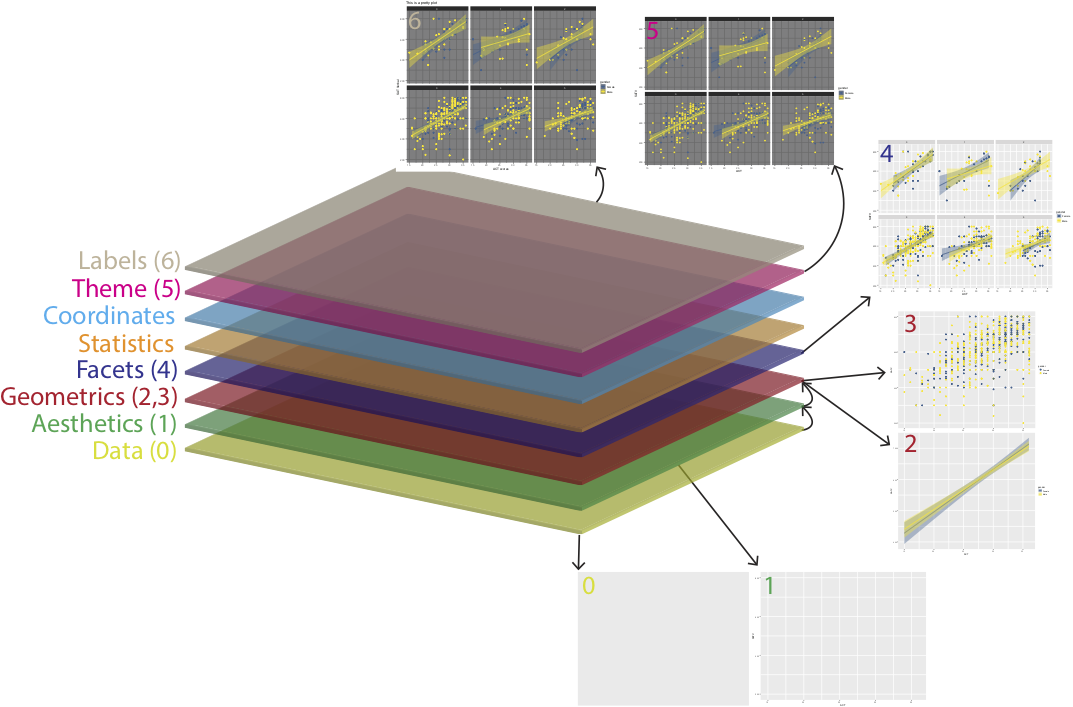
\includegraphics[width=1.0\linewidth,height=0.8\textheight,keepaspectratio]{resources/ggplot_grammar.png}
        \end{figure}
    \end{columns}
\end{frame}

\begin{frame}{Visualization Advice}
    \begin{itemize}
        \item No double Y-axes $\rightarrow$ Very misleading.
        \item Maximize the \href{http://www-personal.umich.edu/~jpboyd/eng403_chap2_tuftegospel.pdf}{'Data-Ink-Ratio'} $\rightarrow $ Keep it simple.
        \item use themes like \texttt{theme\_bw()} to make figures consistent.
        \item thick/horizontal lines to highlight, no or muted tick lines
        \item Think about aspect ratio of your presentation (on Zoom it's usually 16:9, while in-person it's often 4:3) versus write-up. Often need to make axes titles larger than defaults.
    \end{itemize}
\end{frame}


 \begin{frame}{Tips \& Tricks I}
 \begin{itemize}
 \item Start early!!!
 \item[]
 \item Don't oversell your data.
 \item Communicate well with your team, your mentor, your company.
 \item Robustness checks, Validity tests, Simplicity (start with a baseline).
 \item Clean, consistent figures and formatting.
 \item Practice for your final presentation.
 \end{itemize}
 \end{frame}
 
 
 \begin{frame}{Tips \& Tricks II}
\begin{itemize}
    \item Use flags in the header of your script to set constant variables, i.e. path/file names, etc.
    \item Keep a diary of what you've tried. Spending $<2$ Minutes per day on this is already enough and really helps.
    \item Read the documentation.
    \item Use github for version control (especially good with team mates).
    \item Proper motivation and embedding in existing literature or context for final write-up.
 \item Cite references (use citation management like Zotero or Mendeley).
\end{itemize}
 \end{frame}

\section{Q \& A}
\begin{frame}{Q \& A}
\begin{wideitemize}
\item These were just very general points, vocab, and code snippets to get you started.
\item While there's a lot to learn and do, don't feel overwhelmed. A lot of the material here may not apply to your specific project.
\item There are incredible online resources - use them!
\item[]
\item You can always talk to you mentors!
\end{wideitemize}
\end{frame}


\begin{frame}{}
\vspace*{\fill}
\centering \Large \emph{Thank You!} 
\vspace*{\fill}

For feedback, questions, or comments, \\ please email me: ssteffen@mit.edu \\
\url{sebastiansteffen.com}
\end{frame}
\end{document}